% http://www.ctan.org/tex-archive/macros/latex/contrib/beamer/examples
% http://latex.artikel-namsu.de/english/beamer-examples.html

\documentclass{beamer}
\usepackage{amsmath}
\usepackage{amssymb}
\usepackage{bm}
\usepackage{fancybox, graphicx}
\usepackage{listings}
\usepackage{tikz} % Diagrams
\usepackage{color}
\usepackage{textcomp} % See https://tex.stackexchange.com/questions/145416/how-to-have-straight-single-quotes-in-lstlistings

\lstset{language=Python,upquote=true} % Format listings as appropriate for Python. Inexplicably we get problems if the language is set as part of the \begin{lstlisting} command.



\usetheme{boxes}
\usecolortheme{beaver}


\title[IT Workshops] % (optional, use only with long paper titles)
{Introduction to IT for UCL Astrophysicists}

\author{L.~Whiteway, E.~Edmondson, L.~Lucie-Smith, W.~Jennings}

\institute[UCL]
{
  Astrophysics Group\\
  Department of Physics and Astronomy\\
  University College London
}
\date
{17 October 2017}

\subject{IT}

\begin{document}

\frame{\titlepage}

\section{Introduction}

\begin{frame}{Where to find this presentation}
  \begin{block}{}
    Find the presentation at \alert{\url{https://tinyurl.com/y8lyyg5r}}.\\
    Note that the third character is a lower-case `el'. \\
    On this page click on `Download' to get a copy of the presentation.
  \end{block}
\end{frame}


\begin{frame}{Overall goals of presentation}
  \begin{itemize}
    \item What software you might find useful
    \item Pointers to where to get more information (UCL courses, web, etc.)
    \item UCL-specific information (e.g. login details)
    \item Hands-on work
  \end{itemize}
\end{frame}

\begin{frame}{Specific contents}
  \begin{itemize}
    \item Accessing Astrophysics group machines
    \item Using the Linux console
    \item Basics of Python
    \item Commonly used programs (LaTeX, DS9, IRAF,...)
    \item Using High-Performance Computing (HPC) machines
    \item HPC best practices
  \end{itemize}
\end{frame}

\begin{frame}{Information on the Web}
  \begin{block}{Astrophysics Wiki}
    \url{https://wiki.ucl.ac.uk/display/PhysAstAstPhysGrp/Main+Page}
    This Wiki is freely viewable and editable by all members of the department. Please use it to record information that you think will be useful to others (including your future self). Be bold!
  \end{block}

  \begin{block}{UCL Research Computing Platforms}
    \url{https://wiki.rc.ucl.ac.uk/wiki/Main_Page}
  \end{block}
  
  \begin{block}{Stack Overflow}
    \url{http://stackoverflow.com/}
  \end{block}
  
\end{frame}



\begin{frame}{Computing Environment for Astrophysics}
  \begin{itemize}
  \item Large datasets requiring substantial processing followed by sophisticated statistical analysis
  \item Calculations often done on specialised `high-performance computing' (HPC) machines having large filesystems and large RAM; calculations are often broken into pieces that can be run simultaneously (`in parallel') across many processors.
  \item Much useful software is made freely available within the community. Software quality is usually high; documentation quality is more variable.
  \item Many users write their own software.
  \end{itemize}
\end{frame}

\begin{frame}{Local Computing Environment}
  \begin{block}{You will have your own local machine, which might be:}
    \begin{itemize}
      \item PC (Windows)
      \item Mac
      \item Linux
    \end{itemize}
  \end{block}
  \begin{block}{Also there are shared Linux machines:}
    \begin{itemize}
      \item General purpose Astrophysics server available from outside UCL: \alert{\texttt{zuserver1}}
      \item UCL Cosmology HPC cluster: \alert{\texttt{splinter}}
      \item Other UCL HPC clusters: \alert{\texttt{Grace}} and \alert{\texttt{Legion}}
      \item National HPC cluster: \alert{\texttt{DiRAC}}
    \end{itemize}
  \end{block}
\end{frame}

\begin{frame}{Work patterns}
  \begin{block}{Several work patterns are possible:}
    \begin{itemize}
      \item Write and test a program on your local machine; use the local machine to remotely connect to \texttt{splinter}; upload the program to \texttt{splinter} and run it there;
      \item Or do all your work locally (requires small data sets);
      \item Or use the local machine to remotely connect to \texttt{splinter} and do all your work there.
    \end{itemize}
  \end{block}
\end{frame}

\begin{frame}{Remote connections}
  \begin{block}{How to connect to a shared machine}
    \begin{itemize}
      \item Windows PC: use PuTTY;
      \item Mac: go to the Terminal window and use \texttt{ssh};
      \item Linux machine: go to the Terminal window and use \texttt{ssh}.
    \end{itemize}
  \end{block}
  \begin{block}{Visibility}
    If you are not on the UCL network then you cannot connect to \texttt{splinter} directly; instead you must go via \texttt{zuserver1}.
  \end{block}
\end{frame}


\begin{frame}{Two methods for accessing splinter}
  \begin{figure}
    \begin{center}
      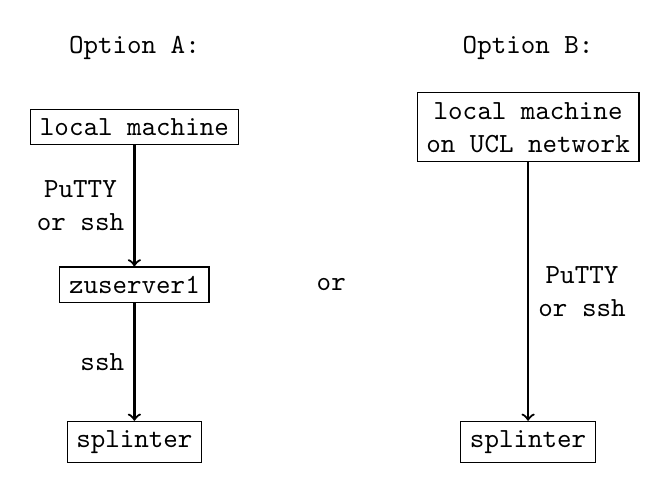
\begin{tikzpicture}[font=\ttfamily]
        \node at (-2.5, 6) {Option A:};
        \node at (2.5, 6) {Option B:};
        \node (LM1) at (-2.5,5) [rectangle,draw] {local machine};
        \node (Z) at (-2.5,3) [rectangle,draw] {zuserver1};
        \node (S1) at (-2.5,1) [rectangle,draw] {splinter};
        \node (LM2) at (2.5,5) [rectangle,draw,align=center] {local machine \\ on UCL network};
        \node (S2) at (2.5,1) [rectangle,draw] {splinter};
        \node at (0,3) {or};
        \draw [->,thick] (LM1.south) -- (Z.north) node [midway,left,align=center] {PuTTY \\ or ssh};
        \draw [->,thick] (Z.south) -- (S1.north) node [midway,left] {ssh};
        \draw [->,thick] (LM2.south) -- (S2.north) node [midway,right,align=center] {PuTTY \\ or ssh};
      \end{tikzpicture}
    \end{center}
  \end{figure}
\end{frame}

\begin{frame}{Accessing remote machines}
  \begin{block}{Credentials}
    \begin{itemize}
      \item You will need a \textit{username} and \textit{password} for \texttt{splinter} (and, if you are using Option A, for \texttt{zuserver1} as well).
      \item If you do not have these already then we can give guest credentials to be used during this course.
    \end{itemize}
  \end{block}
  \begin{block}{The full names of the servers are:}
    \begin{itemize}
      \item \texttt{zuserver1.star.ucl.ac.uk}
      \item \texttt{splinter-login.star.ucl.ac.uk}
    \end{itemize}
  \end{block}
\end{frame}


\begin{frame}{Using PuTTY for remote connections from Windows}
  \begin{itemize}
    \item If you don't have PuTTY you can download it from \url{http://www.putty.org/}.
    \item On the `Connection/SSH/X11' tab, click on `enable X11 forwarding' and set `X display location' to `localhost:0' - this is necessary for handling graphical output.
    \item On the Session tab, set the Host Name as appropriate: \texttt{zuserver1.star.ucl.ac.uk} (Option A) or \texttt{splinter-login.star.ucl.ac.uk} (Option B).
  \end{itemize}
\end{frame}

\begin{frame}{Using ssh for remote connections from Mac and Linux}
  \begin{itemize}
    \item Syntax: \alert{\texttt{ssh -YC username@servername}}
    \item The `Y' option is necessary for handling graphical output.
  \end{itemize}
\end{frame}

\begin{frame}{X-Windows client}
  \begin{itemize}
    \item If the remote program that you are running produces graphical output, then you must have a program (an `X-Windows client') running on your local machine to display this graphical output.
    \item On Windows you can use XMing (\url{https://sourceforge.net/projects/xming/}) or Exceed (available on the UCL Desktop).
    \item On Mac you can use XQuartz.
    \item On Linux you don't need to do anything special - the graphical interface is already an X-server.
  \end{itemize}
\end{frame}


\section{Linux}

\begin{frame}{Linux: Command shell}
  \begin{itemize}
    \item{In Linux you will use a `command shell'.}
    \item{This is a text-based environment in which you type commands and receive text output.}
    \item{Not GUI! Reflects the hardware limitations current when Unix was created. Low-tech and reliable e.g. for remote access.}
    \item{Various command shell programs are used: \texttt{bash}, \texttt{csh}, \texttt{tcsh}, etc. To see which one you are using, call \texttt{echo \$0}.}
   \end{itemize}
\end{frame}

\begin{frame}{Linux: Directory structure}
  \begin{itemize}
    \item{Everything is organised around files (which may be data files or program files i.e. instructions to be executed).}
    \item{Files live in directories. There is a hierarchical tree structure of directories.}
    \item{Sample file name: \texttt{/share/splinter/ucapwhi/des/foo.txt}}
    \item{Note use of slash `/', not backslash `\textbackslash' as in Windows.}
    \item{Case sensitivity: `Foo' and `foo' are different strings.}
  \end{itemize}
\end{frame}

\begin{frame}{Linux: Special symbols for directories}
  \begin{table}[ht]
    \centering
    \begin{tabular}{c l}
      \\ [-2ex]
      Symbol & Meaning \\ [.5ex]
      \hline \\ [-2ex]
      / & Top of the directory tree (the root directory) \\
      . & Current directory \\
      .. & Parent of the current directory \\
      \textasciitilde & User's `home' directory \\ \\
      (TAB) & (Perform autocomplete on directory and file names) \\
    \end{tabular}
  \end{table}
\end{frame}


\begin{frame}{Linux: Environment variables}
  \begin{itemize}
    \item The operating system maintains a global namespace of `environment variables' to store configuration information.
    \item Use \alert{\texttt{printenv}} (in tcsh) or \alert{\texttt{set}} (in bash) to see all environment variables; use \alert{\texttt{echo \$<variable\_name>}} to see the value of one environment variable (e.g. \alert{\texttt{echo \$PATH}}).
    \item Use \alert{\texttt{setenv FOO my\_string}} (in tcsh) or \alert{\texttt{export \$FOO=`my\_string'}} (in bash) to set \texttt{FOO}.
    \item Variables \texttt{PATH} and \texttt{PYTHONPATH} are used frequently (to maintain lists of directories in which to search for executable programs and Python modules, respectively).
    \item Linux has no equivalent of the Windows Registry; configuration is done via the directory structure and the environment variables.
  \end{itemize}
\end{frame}



\begin{frame}{Linux: Structure of commands}
  \begin{block}{Structure}
    \texttt{[command] -[option(s)] [argument]}
  \end{block}
  \begin{Examples}
     \texttt{ls -la \\
     mkdir hello\_world \\
     cp hello.cpp new\_hello.cpp} \\
  \end{Examples}
\end{frame}

\begin{frame}{Linux: command reference}
There is a very useful summary of Linux commands at: \\
\url{http://www.computerhope.com/unix.htm}
\end{frame}


\begin{frame}{Linux: Basic commands 1}
  \begin{columns}
    \column{.5\textwidth}
    \begin{block}{navigation and help}
      \texttt{pwd} \\
      \texttt{ls -la} \\
      \texttt{cd dir\_name} \\
      \texttt{man command\_name} \\
      \texttt{info command\_name} \\
      \texttt{exit}
    \end{block}
    \begin{block}{copy or move}
      \texttt{cp src dest} \\
      \texttt{mv src dest} \\
      \texttt{scp usr@host:file dest}
    \end{block}

    \column{.5\textwidth}
    \begin{block}{create or delete}
      \texttt{touch file.txt} \\ 
      \texttt{mkdir dir\_name} \\ 
      \texttt{rm -i file.txt}
    \end{block}
    \begin{block}{find and system info}
      \texttt{whereis file} \\
      \texttt{which} \\
      \texttt{echo \$VAR\_NAME}
    \end{block}
    \begin{block}{file contents}
      \texttt{cat file} \\
      \texttt{more file} \\
      \texttt{head file}
    \end{block}    
  \end{columns}
\end{frame}


\begin{frame}{Linux: Basic commands 2}
  \begin{columns}
    \column{.5\textwidth}
    \begin{block}{special characters}
      \texttt{\& (background)} \\
      \texttt{; (combine)} \\
      \texttt{\textbackslash$\,$ (next line)} \\
      \texttt{* (wildcard)} \\
      \texttt{| (pipe)} \\
      \texttt{> (output)} \\            
      \texttt{< (input)}
    \end{block}
    \begin{block}{text editors}
      \texttt{emacs} \\
      \texttt{vi} \\
      \texttt{gedit}
    \end{block}

    \column{.5\textwidth}
    \begin{block}{process management}
      \texttt{kill}, \texttt{top}, \texttt{nohup}
    \end{block}    
    \begin{block}{compressed files}
      \texttt{gunzip}, \texttt{tar} 
    \end{block}
    \begin{block}{images}
      \texttt{gthumb} \\
      \texttt{ds9} \\
      \texttt{evince} \\
      \texttt{eog}
    \end{block}    
    \begin{block}{publishing}
      \texttt{latex}, \texttt{bibtex} 
    \end{block}
  \end{columns}
\end{frame}


\begin{frame}[allowframebreaks,t]{Linux: Exercises}
  \begin{enumerate}
    \item Go to your home directory and create a directory called \texttt{level\_0}.
    \item Change directory to \texttt{level\_0}.
    \item Find the name of the present working directory.
    \item Make a directory \texttt{level\_1}, and move to it.
    \item Create a file called \texttt{foo.txt} with contents ``This file contains the word bar''.
    \item Add another line in \texttt{foo.txt} with contents ``This is the second line''.
    \item Print the contents of \texttt{foo.txt} to the screen.
    \item Search for the word \emph{bar} in \texttt{foo.txt}.
    \item Go up one level, then remove the directory \texttt{level\_1} (and its contents).
    \item Find the location of your python installation.
    \item Find the values of the environment variables \texttt{PATH} and \texttt{LD\_LIBRARY\_PATH}.
    \item Set the environment variable \texttt{MY\_VAR} to equal the absolute path to \texttt{level\_0}, and test that it has worked OK.
    \item Add (i.e append) to the \texttt{PATH} the absolute path to \texttt{level\_0}, and test that it has worked OK.
    \item Use the \texttt{man} command to find the option of \texttt{ls} that shows file sizes in human readable format.
    \item Find the hostname, processor type and operating system version and write this info into a text file called \texttt{info.txt}.
    \item List the people who are currently logged into the system.
    \item Find which process is using the most CPU at the moment.
    \item Find the IDs of the processes that you are running.
  \end{enumerate}
\end{frame}

\section{Programming}
\subsection{Python}


\begin{frame}{Programming: Languages}
  \begin{block}{High-level languages - fast to code}
    \begin{itemize}
      \item Python
      \item IDL
      \item Matlib, Mathematica, R
    \end{itemize}
    \end{block}
    \begin{block}{Low-level languages - fast to run}
    \begin{itemize}
      \item C, C++
      \item Fortran
      \item Assembler
    \end{itemize}
  \end{block}
\end{frame}

\begin{frame}{Python}
  \begin{block}{Python has become popular:}
    \begin{itemize}
      \item Good trade-off between ease-of-use and performance
      \item Many add-in libraries, so sophisticated programs can often be built easily [\url{https://xkcd.com/353/].}
    \end{itemize}
  \end{block}
\end{frame}

\begin{frame}{Python Features and Aspects}
  \begin{itemize}
    \item Two slightly-incompatible versions: 2 and 3 (currently 2.7 and 3.6). Still lots of users of 2; better to use 3 if you can.
    \item Can be used interactively or compiled.
    \item Duck typing (type of variable is inferred at run-time)...
    \item ... and hence generic programming (in which a function can take many different types of variables as inputs).
    \item Object-orientation.
    \item Exceptions (try, raise, except) for handling error conditions.
    \item Automatic garbage collection (so no need to worry about memory management).
  \end{itemize}
\end{frame}


\begin{frame}{Python for Astrophysicists}
  \begin{block}{Use Python plus the following add-in libraries:}
    \begin{itemize}
      \item Numpy: array processing for numbers and strings
      \item Scipy: scientific library
      \item Astropy: astronomical library
      \item Matplotlib: plotting
    \end{itemize}
  \end{block}
  \begin{block}{All of these libraries (plus many others) are available in one package called Anaconda:}
    \url{https://www.continuum.io/downloads}.
  \end{block}
\end{frame}

\begin{frame}{Using Python on \texttt{splinter}}
  \begin{itemize}
    \item To initialize your \texttt{splinter} session so that it will use Python 3 and so that it can find all the necessary libraries, run: \\
    \alert{\texttt{module~load~dev\_tools/oct2016/python-Anaconda-3-4.2.0}}
    \item This will set the necessary environment variables.
    \item We will explain in more detail later about the \texttt{module} command.
  \end{itemize}
\end{frame}

% Note that frame must be fragile if we are using lstlisting.
\begin{frame}[fragile]{Python: Interactive}
  \begin{itemize}
    \item Begin an interactive Python session by calling \alert{\texttt{ipython}}
    \item You can then type Python commands on successive lines, such as
  \end{itemize}
  \begin{lstlisting}
        print 2+2
        a = 7
        print a**2
        exit
  \end{lstlisting}
\end{frame}

\begin{frame}{Python: Compiled}
  \begin{itemize}

  \item {Create a Python program by writing code in a text file (say called my\_program.py).}
  \item {Then execute the program by calling \alert{\texttt{python~my\_program.py}}}
  
  \item {Even better:
  \begin{itemize}
   \item Put \alert{\texttt{\#!/usr/bin/env~python}} as the first line in my\_program.py
   \item Run \alert{\texttt{chmod +x~my\_program.py}}
  \end{itemize}
  Then execute the program by calling \alert{\texttt{./my\_program.py}}}
  \end{itemize}
\end{frame}

% Note that frame must be fragile if we are using lstlisting.
\begin{frame}[fragile]{Python: sample program}
  \begin{lstlisting}
  #!/usr/bin/env python
  # Use the `#' to indicate a comment
  
  # Import library and give it a 
  # short name for convenience
  import numpy as np
  
  
  a = np.arange(10) # The array [0, 1, ..., 9]
  b = f(a) # f is a subroutine defined below
  print b
  
  def f(x): 
      # The whitespace at the beginning
      # of the next line is crucial.
      return x**2 
  
  \end{lstlisting}

\end{frame}


% Note that frame must be fragile if we are using lstlisting.
\begin{frame}[fragile]{Python}
  \fontsize{10pt}{10}\selectfont
  \begin{block}{Dictionaries}
  	Useful to do key-value mapping and can be created using \texttt{dict()} \\
  	Can access keys using \texttt{dictionary.keys()} and values using \texttt{dictionary.values()} or \texttt{dictionary[key]}
  \end{block}
  \begin{block}{Functions}
       \begin{lstlisting} 
def function_name(arg1, arg_opt=1, *args, **kwargs):
       \end{lstlisting}
       \texttt{arg\_opt} is an optional argument, and if you don't want to specify the number of arguments use \texttt{*args} for a list of arguments and \texttt{**kwargs} for a dictionary. Example:
       \begin{lstlisting}
function_name(100.0, *[1, 2, 3], **{`foo':`bar'})
       \end{lstlisting}
  \end{block}
  \begin{block}{Classes}
       Can create objects with functions, but must initialise the arguments:
       \begin{lstlisting}
class class_name:
    def __init__(self, arg):
        self.argument = arg
       \end{lstlisting} 
  \end{block}
\end{frame}

\begin{frame}{NumPy}
  \fontsize{9pt}{9}\selectfont
  \begin{block}{NumPy Arrays}
      Can create NumPy arrays in many ways; \texttt{np.array([])}, \texttt{np.empty(())}, \texttt{np.zeros([])}, \texttt{np.ones([])}, \texttt{np.arange()}, \texttt{np.linspace()}, ...
  \end{block}
  \begin{block}{Basic Statistics}
     \texttt{np.mean()}, \texttt{np.median()}, \texttt{np.min()}, \texttt{np.max()}, \texttt{np.std()}, \texttt{np.argmin()}, \texttt{np.argmax()}
  \end{block}
  \begin{block}{Shape Manipulation}
    Can change arrays to be different shapes and size; \texttt{np.reshape()}, \texttt{np.flatten()}, \texttt{np.shape()}, array slicing (next slide...)
  \end{block}    
  \begin{block}{Sorting}
     Can use \texttt{np.sort()} to sort arrays along different axes, and \texttt{np.argsort()} to return the arguments of the sorted arrays
  \end{block}    
  \begin{block}{I/O}
     Can use \texttt{np.loadtxt()} and \texttt{np.genfromtxt()} to get values from a data files. Can choose data type, delimiter, to skip header/footer/rows, to unpack the data into multiple variables, etc. 
  \end{block}     
\end{frame}

\begin{frame}{Array Slicing}
    \texttt{a = np.arange(60).reshape(6,10)[:,0:6]} \\
    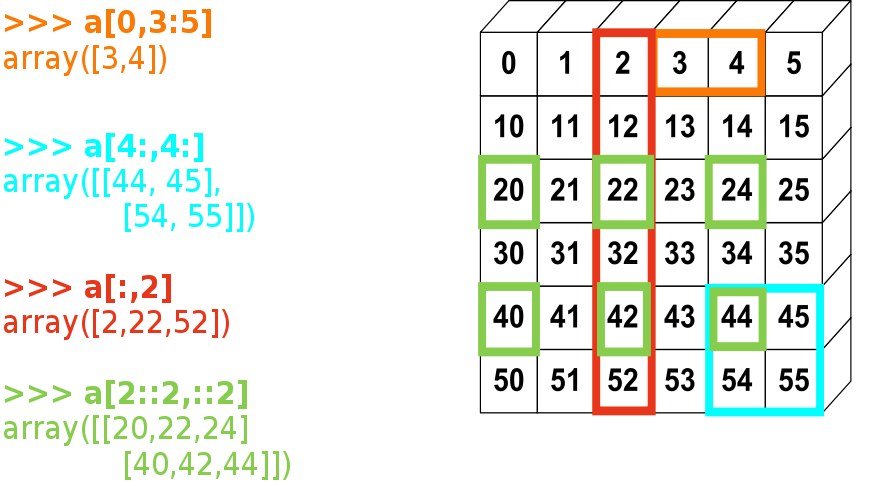
\includegraphics[scale=0.45]{slicing.png}
\end{frame}

\begin{frame}{Scipy/Astropy/PyFITS/SymPy}
  \fontsize{8pt}{8}\selectfont
  \begin{block}{Constants and Conversions}
     For example: \texttt{scipy.constants.c, scipy.constants.hbar, scipy.constants.lambda2nu(550*scipy.constants.nano)}
  \end{block}
  \begin{block}{More Stats}
     Various stats tool using \texttt{scipy.stats}, such as calculating mean, variance, skew, and probability and cumulative density functions
  \end{block}
  \begin{block}{Optimising and Fitting}
      Can use \texttt{scipy.optimize} to find minima (\texttt{.fmin\_bfgs}), find roots of a function (\texttt{.fsolve}), and fitting (\texttt{.curve\_fit})
  \end{block}  
  \begin{block}{PyFits}
      Using \texttt{pyfits}, can import (\texttt{.open()}), read (\texttt{.info()}/\texttt{.header()}), and write (\texttt{.PrimaryHDU()} and \texttt{.writeto()}) FITS files 
  \end{block}  
  \begin{block}{World Coordinate Systems}
      Can find the RA and Dec of pixels using \texttt{astropy.wcs.WCS} and and convert RA and Dec to pixels using \texttt{astropy.wcs.WCS.wcs\_sky2pix()}
  \end{block}
  \begin{block}{Symbolic Calculus}
    Differentiation, Integration, Linear Algebra, Series Expansion, and Equation Simplifying using \texttt{sympy}
  \end{block}
\end{frame}

\begin{frame}{Information on the Web}
  \begin{block}{Documentation}
    \url{http://scipy.org/} \\
    \url{http://matplotlib.org/} \\
    \url{http://www.astropy.org/}
  \end{block}

  \begin{block}{SciPy Tutorials (Also NumPy and Matplotlib)}
    \url{https://conference.scipy.org/scipy2013/tutorials.php}
  \end{block}
  
  \begin{block}{SciPy Lectures (Also NumPy and Matplotlib)}
    \url{http://www.scipy-lectures.org/}
  \end{block}
  
  \begin{block}{Stanford's Introduction to Scientific Python}
    \url{http://web.stanford.edu/~arbenson/cme193.html}
  \end{block}
  
\end{frame}

\begin{frame}{Matplotlib}
  \begin{itemize}
    \item Powerful plotting library. See \url{http://matplotlib.org/gallery.html} for range of examples.
    \item Two interfaces: one similar to MATLAB (for interactive use; relies on global state), and one object-oriented. Typically the latter is to be preferred.
    \item Read the introduction at \url{http://matplotlib.org/faq/usage_faq.html} as this clarifies many points of terminology and usage.
    \item Alas the documentation could be better. StackOverflow clarifies many of the more subtle points.
  \end{itemize} 
\end{frame}



% Note that frame must be fragile if we are using lstlisting.
\begin{frame}[fragile]{Matplotlib Example}
  \begin{lstlisting}

    import numpy as np
    import matplotlib.pyplot as plt
  
    x = np.arange(0, 2*np.pi, 0.1)
    y = np.sin(x)
  
    plt.figure()
    plt.scatter(x, y) # Or plt.plot...
    plt.show()
  
  \end{lstlisting}
\end{frame}

\begin{frame}[fragile]{Matplotlib Features}
  \fontsize{11pt}{11}\selectfont
  \begin{block}{Different Plotting Styles}
     Can edit marker style, colour, edge colour, size and opaqueness, errorbar style and colour. \\
     Can annotate plots with text and arrows. \\
     Can include colour maps and bars (see next slide). \\
     Can plot in polar and World Coordinate System coordinates (with the help of \texttt{astropy}).
  \end{block}
  \begin{block}{Image Plotting}
     Can read and plot an image using \texttt{plt.imshow}. Beware of orientation!
  \end{block}
  \begin{block}{Multiple Subplots}
     Using \texttt{plt.subplot()} you can create multiple subplots, for example the following creates two side-by-side subplots that share x and y axes:\\
     \begin{lstlisting}
plt.subplots_adjust(hspace=0.5)
ax1 = plt.subplot(121)
ax2 = plt.subplot(122, sharex=ax1, sharey=ax1)
     \end{lstlisting}
  \end{block}
\end{frame}

\begin{frame}{Matplotlib Colormaps}
  \begin{itemize}
    \item Plotting mutiple-dimensional data is hard. You can use colour to indicate one of the data dimensions e.g. a contour map with colour shading for elevation above and below sea level.
    \item This requires a mapping (a `colormap') that associates a colour with each data value. The Matplotlib default way of doing this is `rainbow': map data values to wavelength (between `red' and `blue'). This is simple, elegant, physically well-motivated...
    \item ... but suboptimal in practice (because human perception of colour is complicated and involves non-linearities).
    \item Don't use the default colormap; instead, explicitly specify an alternative (\url{https://matplotlib.org/examples/color/colormaps_reference.html}). See also \url{http://www.research.ibm.com/people/l/lloydt/color/color.HTM}.
  \end{itemize}

\end{frame}

\begin{frame}[allowframebreaks,t]{Matplotlib: Exercises}

  \begin{itemize}

    \item Use the SDSS data file (compressed FITS format) \texttt{/share/splinter/ucapwhi/Linux\_training/demo.fits.gz}.
  
    \item Use the pyfits library (\texttt{import astropy.io.fits as pyfits}) to manipulate file columns as numpy arrays.
  
    \item Use the \texttt{open} command to get a handle to the file (\texttt{h = pyfits.open(...)}). Then get e.g. the \texttt{Dist} column via \texttt{x = h[1].data.field(`Dist')}.
    
    \end{itemize}
    
    \begin{enumerate}
  
    \item Create a scatter plot of distance (\texttt{`Dist'}) as a function of r-band absolute magnitude (\texttt{`rMAG'}). Do you think that this data set is a subset of a larger data set?
  
    \item Make a map by scatter-plotting declination (\texttt{`DEdeg'}) as a function of right ascension (\texttt{`RAdeg'}). Use small dots. Why is the density lower at the top? Why should the plot really be flipped left/right?
  
    \item Use astropy to redo the last plot so that it uses an equal area all-sky projection such as `mollweide'.
    
  \end{enumerate}
\end{frame}

\begin{frame}{Jupyter}
  Jupyter is a framework for creating interactive web pages in which source code (written in Python or other high-level language) appears together with the corresponding output (text or graphics). This is an excellent environment for demonstrating how your code works.\\
  See \url{http://jupyter.org/}.
\end{frame}

\begin{frame}{UCL Software Carpentry Workshop}
  \begin{block}{UCL training course in programming skills}
    \url{https://www.ucl.ac.uk/isd/services/research-it/training}
  \end{block}
  \begin{block}{Upcoming courses}
    \begin{itemize}
      \item 31st October - 1st November 2017
      \item 14th - 15th December 2017
    \end{itemize}
  \end{block}
\end{frame}


\begin{frame}{Source control system}
  \begin{itemize}
    \item A source control system is a repository for successive versions of documents (e.g. source code for computer programs).
    \item Versions can be compared and old versions restored if needed (e.g. to undo recent bad changes).
    \item Multiple developers are able to make changes to the same file, with automatic merging of edits from different developers (but if there is an \textit{edit conflict} i.e. two developers change the same line then manual intervention will be needed).
    \item Any serious development that you do (even if just for yourself) should be under the control of a source control system.
  \end{itemize}
\end{frame}
    
\begin{frame}{Git}
  \begin{itemize}
    \item We often use the source control system `Git'.
    \item Git is non-trivial to learn (see \url{https://xkcd.com/1597/}) but is very powerful. It is useful to have a clear idea of Git's internal workings before attempting to do even simple things.
    \item Git uses a `distributed' model (as opposed to a `client/server' model used e.g. by SVN). All copies of a repository are `peers' (i.e. no one copy is special as far is Git is concerned).
  \end{itemize}
\end{frame}

\begin{frame}{Git workstyles}
  \begin{itemize}
    \item Git can be used in support of various work styles.
    \item For most projects that you will encounter, it is sufficent to put a repository somewhere on the Internet and think of this as the  `official' copy. You can then `clone' this repository locally, make your changes, and then `push' this pack to the official repository. Your colleagues will be doing the same, and Git will handle the necessary merging.
    \item On larger projects you begin by copying the official repository to a new `forked' copy (also on the Internet). You can then develop (as above) in this fork. Later you can ask for your forked copy be merged back into the official copy (`pull request'). This gives the official owners more control over changes.
  \end{itemize}
\end{frame}

%\begin{frame}{Git: Picture}
%  \begin{figure}
%    \begin{center}
%      \begin{tikzpicture}[font=\ttfamily]
%        \node (U) at (-5.5,5) {Upstairs};
%        \node (D) at (-5.5,1) {Downstairs};
%        \node (M) at (-2,5) [rectangle,draw] {master};
%        \node (CM) at (-2,1) [rectangle,draw] {clone of master};
%        \node (B) at (3,5) [rectangle,draw,align=center] {branch};
%        \node (CB) at (3,1) [rectangle,draw] {clone of branch};
%        \draw [transform canvas={yshift=3pt},->,thick] (M.east) -- (B.west) node [midway,above,align=center] {fork};
%        \draw [transform canvas={yshift=-3pt},->,thick] (B.west) -- (M.east) node [midway,below,align=center] {pull};
%        \draw [transform canvas={xshift=-3pt},->,thick] (M.south) -- (CM.north) node [midway,left,align=center] {clone};
%        \draw [transform canvas={xshift=3pt},->,thick] (CM.north) -- (M.south) node [midway,right,align=center] {push};
%        \draw [transform canvas={xshift=-3pt},->,thick] (B.south) -- (CB.north) node [midway,left,align=center] {clone};
%        \draw [transform canvas={xshift=3pt},->,thick] (CB.north) -- (B.south) node [midway,right,align=center] {push};
%      \end{tikzpicture}
%    \end{center}
%  \end{figure}
%\end{frame}

\begin{frame}{GitHub and BitBucket}    
  \begin{itemize}
  \item GitHub (\url{https://github.com}) and BitBucket (\url{https://bitbucket.org}) make available Internet-accessible storage space for git repositories.
  \item Both give Web Browser access to repositories.
  \item With both you can install Git locally (command-line interface) and both provide a user-friendly GUI interface to the local Git software.
  \end{itemize}
\end{frame}


\section{Common Programs}
\begin{frame}{Common and Useful Programs}
  \begin{itemize}
  \item \LaTeX
  \item DS9
  \item IRAF
  \item SExtractor/SWarp
  \item CosmoSIS
  \end{itemize}
\end{frame}

\begin{frame}{\LaTeX}
  \begin{block}{Features}
    \begin{itemize}
      \item \LaTeX is text processing software.
      \item Not WYSIWYG. Source files are text files (which \LaTeX then compiles into pdf); as a result e.g. it is easy to merge two sets of changes.
      \item Optimised for good display of mathematics.
      \item Required for submissions to arXiv.
      \item Use `beamer' to produce presentations (e.g. this one).
      \item Use `tikz' to produce diagrams (as in this presentation).
    \end{itemize}
  \end{block}
  \begin{block}{Websites}
    \url{http://www.tug.org/texworks/}
  \end{block}
\end{frame}

\begin{frame}{DS9}
  \begin{block}{Features}
   \begin{itemize}
    \item{Viewer for FITS and othjer files}
    \item{Aligning with WCS (World Coordinate System)}
    \item{Scaling image contrast}
    \item{Funky colour sets (and inverse or negative)}
    \item{Regions and annotating the image}
    \item{Multiple frames; blinking and matching}    
    \item{Contour plots}
  \end{itemize}
  \end{block}
  \begin{block}{Website}
    \url{http://ds9.si.edu/site/Home.html}
  \end{block}
\end{frame}

\begin{frame}{Image Reduction and Analysis Facility (IRAF)}
  \begin{block}{Features}
   \begin{itemize}
   \item{\textit{`IRAF is a collection of software geared towards the reduction of astronomical images in pixel array form ... from imaging array detectors such as CCDs.'}}
   \item{\textit{`IRAF commands (known as tasks) are organized into package structures. Additional packages may be added to IRAF. There are many packages ... focusing on a particular branch of research or facility.'}}
   \item{ Example package: STSDAS (for analysing Hubble Space Telescope data).}
   \end{itemize}
  \end{block}
  \begin{block}{Websites}
    \url{http://iraf.noao.edu/}\\
    \url{http://iraf.net/irafdocs/}
  \end{block}
\end{frame}

\begin{frame}{SExtractor/SWarp}
  \begin{block}{Features}
   \begin{itemize}
    \item{\textit{`SExtractor is a program that builds a catalogue of objects from an astronomical image. Although it is particularly oriented towards reduction of large scale galaxy-survey data, it can perform reasonably well on moderately crowded star fields.'}}
    \item{\textit{`SWarp is a program that resamples and co-adds together FITS images using any arbitrary astrometric projection defined in the WCS standard.'}}
   \end{itemize}
  \end{block}
  \begin{block}{Websites}
    \url{http://www.astromatic.net/software/sextractor}\\
    \url{http://www.astromatic.net/software/swarp}
  \end{block}
\end{frame}

\begin{frame}{CosmoSIS}
  \begin{block}{Features}
    \begin{itemize}
      \item \textit{`CosmoSIS is a cosmological parameter estimation code. It is a framework for structuring cosmological parameter estimation in a way that eases re-usability, debugging, verifiability, and code sharing in the form of calculation modules. It consolidates and connects together existing code for predicting cosmic observables, and makes mapping out experimental likelihoods with a range of different techniques much more accessible.'}
    \end{itemize}
  \end{block}
  \begin{block}{Websites}
    \url{https://bitbucket.org/joezuntz/cosmosis/wiki/Home}
    \url{https://wiki.ucl.ac.uk/display/PhysAstAstPhysGrp/Installing+and+Running+CosmoSIS}
  \end{block}

\end{frame}

\begin{frame}{ASCL.net}
There's more: the Astrophysics Source Code Library (\url{http://ascl.net/}) lists over 1000 astronomical programs that you can download.
\end{frame}


\section{HPC}

\begin{frame}{HPC: Information on the Web}

    \begin{block}{Introduction to Parallel Computing (Presentation)}
    \url{https://wiki.ucl.ac.uk/display/PhysAstAstPhysGrp/Computing+and+Programming}
  \end{block}

    \begin{block}{UCL Astrophysics Wiki information on \texttt{splinter}}
    \url{https://wiki.ucl.ac.uk/display/PhysAstAstPhysGrp/Splinter+User+Guide}
  \end{block}

  \begin{block}{UCL Research Computing Platforms}
    \url{https://wiki.rc.ucl.ac.uk/wiki/Main_Page}
  \end{block}

  \begin{block}{DiRAC}
    \url{http://www.dirac.ac.uk/}
  \end{block}

\end{frame}

\begin{frame}{HPC: \texttt{splinter} mailing list}
	\url{https://www.mailinglists.ucl.ac.uk/mailman/listinfo/splinter-users}
	\bigskip
	\begin{itemize}
		\item Please subscribe
		\item Post any issues regarding \texttt{splinter}
	\end{itemize}
\end{frame}

\begin{frame}{HPC: Cluster structure}

  A HPC cluster (such as \texttt{splinter}) consists of many nodes (= `boxes' = machines).
  \begin{itemize}
    \item One node is the `login' node; it hosts the command session that you get when you log in.
    \item Another node is the `head'; it runs the software that controls how the cluster operates.
    \item All the other nodes are `compute' nodes; they do the actual work.
    \item The nodes can talk to each other via an Ethernet network.
  \end{itemize}

\end{frame}

\begin{frame}{HPC: Node structure}
  Each node has:
  \begin{itemize}
    \item Several cores  (= processors). Each core can run computer code independently of each other.
    \item Memory (RAM) that can be allocated to the cores. If necessary some memory can be used by several cores at once.
    \item Its own file space.
  \end{itemize}
\end{frame}


\begin{frame}{HPC: \texttt{splinter} nodes and cores}
	Currently \texttt{splinter} has 29 nodes and 456 cores:
	\begin{itemize}
		\item 8 nodes each with 12 cores and 48GB RAM
		\item 20 nodes each with 16 cores and 128GB RAM
		\item 1 node with 40 cores and 1TB RAM
	\end{itemize}
\end{frame}

\begin{frame}{HPC: Program structure}
  \begin{itemize}
    \item A simple program runs code sequentially using just one core.
    \item More complex programs run more quickly by running several `threads' of code in parallel on several cores within one node - one thread per core.
    \item So the simple programs are `single-threaded' and the more complex are `multi-threaded'.
    \item A multi-threaded program can run on just one core if necessary - the threads will execute one after another and the program will run more slowly.
  \end{itemize}
\end{frame}

\begin{frame}{HPC: How to parallelize}
  Method 1:
  \begin{itemize}
    \item Write a single-threaded program.
    \item Run many copies of it at once; each uses one core.
    \item Run time depends on total number of cores.
    \item Single-threaded programs are easy to write and debug.
    \item No fast way for the various running copies to talk to each other during processing. Therefore this method is useful only when the problem can be divided into independent chunks. Such problems are called `embarrassingly parallel'.
    \item Easy to submit many jobs at once using a `Job Array' - see \texttt{splinter} user guide.
  \end{itemize}
\end{frame}

\begin{frame}{HPC: How to parallelize}
  Method 2:
  \begin{itemize}
    \item Write a multi-threaded program.
    \item Run it on one node, using all the cores on that node.
    \item Run time depends on maximum number of cores on one node.
    \item Multi-threaded programs are hard to write and debug. Tools called `OpenMP' and `MPI' help.
    \item The threads can share memory hence can talk to each other during processing; for certain problems this is crucial. Need to be careful that the threads don't conflict when updating shared memory.
  \end{itemize}
\end{frame}

%\begin{frame}{HPC: \texttt{splinter} distributed}
%  \begin{figure}
%    \begin{center}
%      \shadowbox{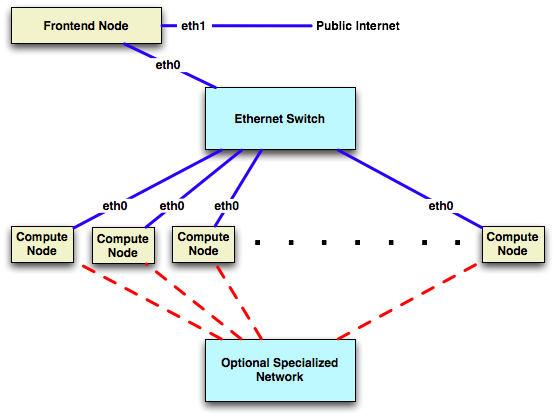
\includegraphics[scale=0.4]{cluster.png}}
%      \footnote{\url{http://www.rocksclusters.org/}}
%    \end{center}
%  \end{figure}
%\end{frame}

%\begin{frame}{HPC: \texttt{splinter} shared}
%  \begin{figure}
%    \begin{center}
%      \shadowbox{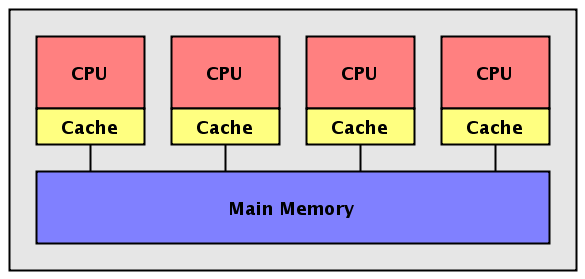
\includegraphics[scale=0.4]{fig03.png}}
%      \footnote{\url{http://www.cs.rit.edu/}}
%    \end{center}
%  \end{figure}
%\end{frame}

\begin{frame}{HPC: Workspaces I}
	\begin{block}{\texttt{/home/user\_name}}
		\begin{itemize}
			\item This is your home directory
			\item Login scripts can be put here
			\item 1GB quota
			\item Private
		\end{itemize}
	\end{block}
	\begin{block}{\texttt{/share/splinter/user\_name}}
		\begin{itemize}
			\item Create the directory if it is not already there
			\item Can be used as a workspace
			\item No quota
			\item Public unless made private
		\end{itemize}
	\end{block}
\end{frame}

\begin{frame}{HPC: Workspaces II}
	\begin{block}{\texttt{/share/data1}}
		\begin{itemize}
			\item For storing large data
			\item You can create a directory for your, .e.g, \texttt{/share/data1/SKA}
		\end{itemize}
	\end{block}

	\begin{block}{\texttt{/share/apps}}
		\begin{itemize}
			\item For installing software
			\item Module files
		\end{itemize}
	\end{block}
\end{frame}

\begin{frame}{HPC: Login script}
  \begin{itemize}
    \item There is a file called \texttt{.login} in your \texttt{\$HOME} directory
    \item Every time you login this file will be executed
    \item You can load modules, envvars, etc.
  \end{itemize}
  \begin{Examples}
    \begin{block}{Load my aliases}
      \texttt{source $\sim$/aliases.csh}
    \end{block}
    \begin{block}{Load python}
      \texttt{module load dev\_tools/oct2016/python-Anaconda-3-4.2.0}
    \end{block}
  \end{Examples}
\end{frame}

\begin{frame}{HPC: Modules}
	\begin{itemize}
		\item A module file sets environment variables required to run a program. This makes it easy e.g. to switch between different versions of a program.
		\item Available to everyone in \texttt{splinter}
	\end{itemize}
	
	\begin{Examples}
	    \begin{columns}
                \column{.5\textwidth}
		\begin{block}{Print the available modules}
			\texttt{module avail}
		\end{block}
		\begin{block}{Load a module}
			\texttt{module load module\_name}
		\end{block}
		\begin{block}{List the loaded modules}
			\texttt{module list}
		\end{block}
	
	        \column{.5\textwidth}
		\begin{block}{Unload a module}
			\texttt{module unload module\_name}
		\end{block}
		\begin{block}{Unload all modules}
			\texttt{module purge}
		\end{block}		
		\begin{block}{Help}
			\texttt{module --help}
		\end{block}	
	    \end{columns}								
	\end{Examples}
\end{frame}

\begin{frame}{HPC: Submitting jobs}
	\begin{itemize}
		\item Computing jobs should be submitted to the scheduler.
		\item To do this you will need to write a `job script'.
		\item Alternatively you can start an interactive session on a compute node.
		\item Don't run heavy programs on the login node!
	\end{itemize}
    \begin{Examples}
	    \begin{columns}
                \column{.5\textwidth}    
		\begin{block}{Submit a job}
			\texttt{qsub job\_script}
		\end{block}
		\begin{block}{Start an interactive session}
			\texttt{qsub -IX}
		\end{block}
		\begin{block}{Check the status of a job}
			\texttt{checkjob job\_id}
		\end{block}

	        \column{.5\textwidth}		
		\begin{block}{List the status of all jobs}
			\texttt{qstat}
		\end{block}
		\begin{block}{Show the queue}
			\texttt{showq}
		\end{block}		
		\begin{block}{Delete a job}
			\texttt{qdel job\_id}
		\end{block}
	    \end{columns}		
    \end{Examples}
\end{frame}

\begin{frame}{HPC: Queues}
  When submitting a job you can specify a queue (= subset of nodes) to ensure that your job is processed only on nodes with sufficient resources. Available queues are:
	\begin{itemize}
		\item \texttt{compute} (all nodes)
		\item \texttt{cores16} (all 16 core nodes)
		\item \texttt{cores12} (all 12 core nodes)
		\item \texttt{smp} (all 40 core nodes (there's only one))
	\end{itemize}
\end{frame}

\begin{frame}{HPC: Structure of a job script}
	\texttt{\#!/bin/tcsh \\
	\#PBS -S /bin/tcsh \\
	\#PBS -q cores12 \\
	\#PBS -N a\_name\_for\_your\_job \\
	\#PBS -l nodes=1:ppn=6 \\
	\#PBS -l mem=32gb \\
	\#PBS -l walltime=120:00:00} \\
	
	\begin{block}{\# Set environment variables if needed}
	    \texttt{setenv OMP\_NUM\_THREADS 6}
        \end{block}
	\begin{block}{\# Load module files if needed}
	    \texttt{module load dev\_tools/oct2016/python-Anaconda-3-4.2.0}
        \end{block}
	\begin{block}{\# Run the program}
	    \texttt{/home/username/hello\_world.exe}
        \end{block}	
\end{frame}

\begin{frame}{HPC: Jobscripts: things to remember}
	\begin{itemize}
		\item Choose the correct queue
		\item Choose the correct number of \texttt{nodes} and \texttt{ppn}
		\item Specify the memory required
		\item Always specify the walltime
		\item If your program is not parallel, please use \texttt{nodes=1,ppn=1}
		\item Use the \texttt{compute} queue for single processor jobs
		\item Use \texttt{qsub -IX} for an interactive session
		\item If using most of the resources, please send an email to the mailing list.
	\end{itemize}
\end{frame}

\begin{frame}{HPC: More PBS commands}
	\begin{block}{Specify output}
	    \texttt{\# PBS -o path/to/file.out}
        \end{block}
	\begin{block}{Specify error output}
	    \texttt{\# PBS -e path/to/file.err}
        \end{block}
	\begin{block}{Mail alert at (b)eginning, (e)nd, and (a)bortion of execution}
	    \texttt{\# PBS -m bea}
        \end{block}
	\begin{block}{Send mail to the following address}
	    \texttt{\# PBS -M your\_email\_id@ucl.ac.uk}
        \end{block}                        
\end{frame}

\begin{frame}{HPC: Using \emph{Ganglia}}
	\url{http://splinter.star.ucl.ac.uk/ganglia/}

	\begin{itemize}
		\item A tool for analysing \texttt{splinter}.
		\item Can only be loaded from \texttt{splinter} (using Firefox).
		\item Will give you load/memory information.
		\item Can look into nodes.
	\end{itemize}
\end{frame}

\begin{frame}{HPC: Collaborative projects}
	\begin{itemize}
		\item For collaborations between two splinter users you can share common data in \texttt{/share/data1/my\_collaboration}
		\item Give read/write permission to other users using \texttt{chmod}
	\end{itemize}
\end{frame}


\begin{frame}{HPC: Best practices}
  \begin{itemize}
    \item Choose the compute nodes that are suited for your problem
    \item Read the User Guide
    \item Do not run your programs in the login node
    \item Install common software locally if and only if absolutely necessary
    \item Request optimum resources
    \item Minimise data transfer between nodes
    \item Backup anything that you would hate to lose
  \end{itemize}
\end{frame}

\begin{frame}{HPC: Exercises}
  \begin{enumerate}
    \item Start an interactive session. Find which node you have been assigned.
    \item Still in the interactive session, run `ipython` and run some Python commands. Then exit ipython and the interactive session.
    \item Write a job script to run a `hello world` program in Python and submit it to the queue.
    \item Amend the job file so that the output goes to a file.
    \item Using the above example, check the job status using `qstat` and `checkjob`.
  \end{enumerate}
\end{frame}

\begin{frame}[fragile]{Extra Slides - Python Examples}
  \fontsize{7pt}{7}\selectfont
  \begin{block}{Dictionary example:}
  \begin{lstlisting}
dc = dict(a=1, b=''Hello World'', c=(1, 2, 3))
print dc.keys(), dc.values(), dc[''b'']
  \end{lstlisting}
  \end{block}
  \begin{block}{Function example:}
  \begin{lstlisting}
def my_first_func(arg1, arg_vol=1, *args, **kwargs):
    print arg1, arg_vol
    for a in args:
        print a
    for key, value in kwargs.iteritems():
        print key, value
  \end{lstlisting}
  \end{block}
  \begin{block}{Class example:}
  \begin{lstlisting}
class my_first_class:
    def __init__(self, arg):
        self.argument = arg

    def print_arg(self):
        return self.argument

instance = my_first_class(42)
print instance.method()
  \end{lstlisting}
  \end{block}
\end{frame}

\begin{frame}[fragile]{Extra Slides - NumPy Examples}
  \fontsize{7pt}{7}\selectfont
  \begin{block}{Shape Manipulation examples:}
  \begin{lstlisting}
a = numpy.arange(60).reshape(6,10)
print a.shape
print a.flatten()
print a.reshape(2, -1, 3)  
  \end{lstlisting}
  \end{block}
  \begin{block}{Sorting examples:}
  \begin{lstlisting}
a = numpy.array([2, 6, 5, 1, 6, 3, 3])
print numpy.sort(a)
print numpy.argsort(a)

data_type = [(''wavelength'', int), (''flux'', float)]
values = [(31, 210), (45, 3400), (18, 150), (7, 50), (21, 100)]
array = numpy.array(values, dtype=data_type)
print numpy.sort(array, order=''wavelength'')
  \end{lstlisting}
  \end{block}
  \begin{block}{I/O examples:}
  \begin{lstlisting}
data = numpy.genfromtxt(file_name, dtype=data_type, 
    delimiter=delimiter_character, skip_header=number_of_lines_to_skip)
data1, data2 = np.loadtxt(file_name, skiprows=number_of_lines_to_skip, 
    unpack=True)
  \end{lstlisting}
  \end{block}
\end{frame}

\begin{frame}[fragile]{Extra Slides - Scipy/Astropy/PyFITS/SymPy Examples 1}
  \fontsize{6pt}{6}\selectfont
  \begin{block}{Constants and conversions example:}
  \begin{lstlisting}
x = scipy.constants.find('Newton')
print scipy.constants.value(x[0]), scipy.constants.unit(x[0])
  \end{lstlisting}
  \end{block}   
  \begin{block}{More stats examples:}
  \begin{lstlisting}
bell = scipy.stats.norm(loc=centre, scale=standard_deviation)
print bell.stats(moments='mvs')
print bell.pdf([value, value_2, value_3])
print bell.cdf([value, value_2, value_3])
  \end{lstlisting}
  \end{block}
  \begin{block}{Optimising and Fitting examples:}
  \begin{lstlisting}
minima1 = scipy.optimize.fmin_bfgs(function, initial_guess)
minima2 = scipy.optimize.brute(function, (search_grid,))

r1 = scipy.optimize.fsolve(function, initial_guess)
r2 = scipy.optimize.newton_krylov(function, initial_guess, verbose=True)

opt_values, covariance_matrix = scipy.optimise.curve_fit(function, x_data, y_data)
plt.plot(x_data, y_data, 'bo', label='data')
plt.plot(x_data, function(x_data, opt_values[0], opt_values[1]), 'r-', label='fit')
  \end{lstlisting}
  \end{block}
\end{frame}

\begin{frame}[fragile]{Extra Slides - Scipy/Astropy/PyFITS/SymPy Examples 2}
  \fontsize{6pt}{6}\selectfont
  \begin{block}{PyFITS examples:}
  \begin{lstlisting}
fh = pyfits.open(file_name)
print fh.info(), fh[1].header()

hdu = pyfits.PrimaryHDU(data)
hdu.writeto(new_image_name, clobber=True) 
  \end{lstlisting}
  \end{block} 
  \begin{block}{World Coordinate System examples:}
  \begin{lstlisting}
wcs = astropy.wcs.WCS(header=pyfits.open(file_name)[1].header)
pixcrd = numpy.array([[coord1_x, coord1_y], [coord2_x, coord2_y]], numpy.float_)
sky = wcs.wcs_pix2sky(pixcrd, 1)
print sky

pixcrd2 = wcs.wcs_sky2pix(sky, 1)
print pixcrd2
  \end{lstlisting}
  \end{block}
  \begin{block}{Symbolic Calculus examples:}
  \begin{lstlisting}
a = sympy.Symbol(''a'')
b = sympy.Symbol(''b'')
e = (a + 2*b)**5
e.diff(b)
sympy.integrate(a**2 * sympy.cos(a), a)
sympy.simplify((a + a*b)/a)
sympy.series(sympy.cos(a), a)
  \end{lstlisting}
  \end{block}
\end{frame}

\begin{frame}[fragile]{Extra Slides - Matplotlib Examples}
  \fontsize{6pt}{6}\selectfont
  \begin{block}{Annotate examples:}
      \url{http://matplotlib.org/examples/pylab_examples/annotation_demo2.html}
  \end{block}
  \begin{block}{Polar and color/size/opaqueness example:}
  \begin{lstlisting}
plt.figure(figsize=(10,10))
ax = plt.subplot(111, polar=True)
c = scatter(angles, radii, c=colors, s=sizes, alpha=opaqueness)
plt.show()
  \end{lstlisting}
  \end{block}
  \begin{block}{Image plot example:}
  \begin{lstlisting}
datafile = matplotlib.cbook.get_sample_data(file_name, asfileobj=True)
A = fromstring(datafile.read(), uint16).astype(float)
A *= 1.0/max(A)
A.shape = 512, 512
im = plt.imshow(A, cmap=cm.hot, origin='upper', extent=plot_size)
plt.show()
  \end{lstlisting}
  \end{block}
  \begin{block}{Subplot and colour bar example:}
  \begin{lstlisting}
fig, axes = plt.subplots(nrows=2, ncols=2)
for dat, ax in zip(data, axes.flat):
    im = ax.imshow(dat, vmin=colour_min, vmax=colour_max)
cax = fig.add_axes([left, bottom, width, height])
fig.colorbar(im, cax=cax)
plt.show()
  \end{lstlisting}
  \end{block}
\end{frame}

\end{document}
